%----------------------------------------
\begin{frame}[fragile]
  \frametitle{Recall: the heater controller's hysteresis} \small
\leanbadge{1}{refuted}{red!75!black}

\vspace{-0.35cm}
\whereami{ctl}

\vspace{-0.1cm}
In automatic mode, every average reading goes through two tests:

\begin{lstlisting}[style=cpp]
if      (avgTemp < (m_targetTemp - m_hysteresis)) newState = ON;   // too cold
else if (avgTemp > (m_targetTemp + m_hysteresis)) newState = OFF;  // too hot
if (newState != m_heaterState) commandHeater(newState);
\end{lstlisting}

\pause
\vspace{0.2cm}

With the defaults, target 25\,$^\circ$C and hysteresis {\bf +2}\,$^\circ$C:

\vspace{0.15cm}
{\centering
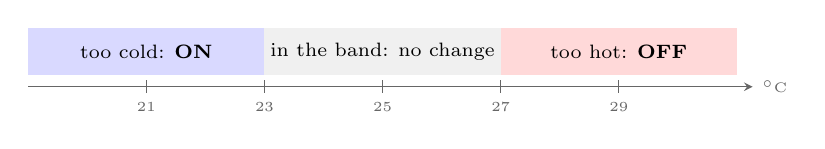
\begin{tikzpicture}[font=\scriptsize, >=stealth]
  \draw[->, black!60] (0,0) -- (9.2,0) node[right, font=\tiny] {$^\circ$C};
  \foreach \x/\t in {1.5/21, 3/23, 4.5/25, 6/27, 7.5/29} {
    \draw[black!60] (\x,0.08) -- (\x,-0.08) node[below, font=\tiny] {\t};
  }
  \fill[blue!15] (0,0.15) rectangle (3,0.75);
  \node at (1.5,0.45) {too cold: {\bf ON}};
  \fill[black!6] (3,0.15) rectangle (6,0.75);
  \node at (4.5,0.45) {in the band: no change};
  \fill[red!15] (6,0.15) rectangle (9,0.75);
  \node at (7.5,0.45) {too hot: {\bf OFF}};
\end{tikzpicture}\par}

\end{frame}
%----------------------------------------
\begin{frame}[fragile]
  \frametitle{A proof attempt that failed --- usefully} \small
\leanbadge{1}{refuted}{red!75!black}

Proposed: {\em ``a hot reading turns the heater off''}.

\begin{lstlisting}[language=lean4]
theorem hot_reading_commands_heater_off (s : ControllerState) (d : AvgTempData)
    (ha : s.controlMode = ControlMode.AUTOMATIC)
    (hc : s.heaterCmdConnected = true)
    (hon : s.heaterState $\neq$ HeaterState.OFF)
    (hhot : s.targetTemp + s.hysteresis < d.avgTemp) :
    let s' := avgTempIn_handler s d
    s'.commandsOut = s.commandsOut ++ [HeaterState.OFF]
\end{lstlisting}

\vspace{-0.15cm}
\pause

{\bf Refuted}, with a counterexample: target 25\,$^\circ$C, hysteresis $-2\,^\circ$C,
heater ON, reading 26\,$^\circ$C.

\begin{itemize}\small
\item 26\,$^\circ$C is hot. But $26 < 25 - (-2)$: it
      also counts as ``too cold'', that test comes first, and the heater stays {\bf on}.

\pause      

\item The C++ avoids this by checking the hysteresis when it is set:
      {\tt SET\_HYSTERESIS} rejects anything below 0.1\,$^\circ$C.
      An invariant is needed: {\tt hysteresis > 0}.
      However, it suggests a {\bf precondition} for the handler.
\end{itemize}

\vspace{-0.1cm}
{\scriptsize A refutation is a finding either way: about the code, or about what we
believed of it.}

\end{frame}

%----------------------------------------
\begin{frame}
  \frametitle{How the actuator keeps track of the heater} \small
\leanbadge{2}{bug found}{red!75!black}

\vspace{-0.35cm}
\whereami{act}

\vspace{-0.1cm}
From the controller to the {\bf actuator}: the component that stops the heater when it
runs too long. Once a second it records whether the heater is on.

\vspace{0.25cm}
{\centering
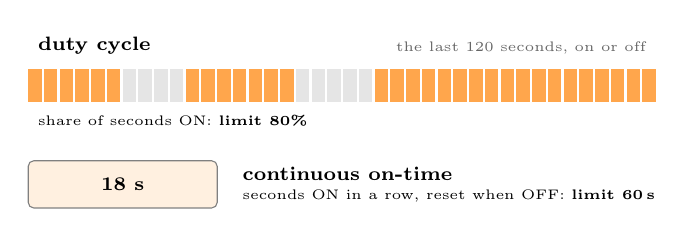
\begin{tikzpicture}[font=\scriptsize, >=stealth]
  % the duty-cycle window: the last 120 seconds, one cell per second (drawn as 40)
  \foreach \i in {0,...,39} {
    \pgfmathsetmacro{\on}{(\i<6 || (\i>=10 && \i<17) || \i>=22) ? 1 : 0}
    \ifdim\on pt=1pt
      \fill[orange!70] (\i*0.2, 0) rectangle ++(0.17, 0.42);
    \else
      \fill[black!10] (\i*0.2, 0) rectangle ++(0.17, 0.42);
    \fi
  }
  \node[anchor=south west, font=\scriptsize\bfseries] at (0, 0.48) {duty cycle};
  \node[anchor=south east, font=\tiny, text=black!60] at (7.97, 0.48)
    {the last 120 seconds, on or off};
  \node[anchor=north west, font=\tiny] at (0, -0.05) {share of seconds ON: {\bf limit 80\%}};

  % the continuous on-time counter
  \draw[rounded corners=2pt, draw=black!50, fill=orange!12] (0,-1.35) rectangle (2.4,-0.75);
  \node[font=\scriptsize\bfseries] at (1.2,-1.05) {18 s};
  \node[anchor=west, font=\scriptsize\bfseries] at (2.6,-0.92) {continuous on-time};
  \node[anchor=west, font=\tiny] at (2.6,-1.2) {seconds ON in a row, reset when OFF:
    {\bf limit 60\,s}};
\end{tikzpicture}\par}

\vspace{0.3cm}
Either limit exceeded: the heater goes to {\bf FAULT}.

\pause
\vspace{0.15cm}

\begin{block}{{\tt RESET\_STATISTICS}, an operator command}\small
Clears the duty-cycle buffer (the last 120 seconds) and sets the on-time counter to 0:
the record of how long the heater has been on is gone.
\end{block}

\end{frame}
%----------------------------------------
\begin{frame}[fragile]
  \frametitle{A proved theorem that was the wrong theorem} \small
\leanbadge{2}{bug found}{red!75!black}

\vspace{-0.3cm}
{\bf 1.}\ \ A violated safety limit leads to FAULT within one second (10 ticks):

\vspace{0.1cm}
\begin{lstlisting}[language=lean4]
theorem tick_sequence_corrects_safety (s) (params) :
  Reachable s params -> violatesSafetyLimits s params ->
  let ticks := List.replicate TICKS_PER_UPDATE SystemEvent.Tick
  (executeTrace params ticks s).currentState = HeaterState.FAULT
\end{lstlisting}

\vspace{-0.05cm}
{\bf Proved.} But the 10 events are {\em only} ticks: nothing else may happen.

\pause

\vspace{0.25cm}
\tikz[remember picture, overlay]{\node[anchor=east] at ([xshift=-0.35cm]current page.east |- 0,0.05) {\ideaicon[0.9]};}%
\parbox{0.86\textwidth}{{\bf 2.}\ \ Corrected: the heater reaches {\bf FAULT} for {\em any} events, as long as
10 of them are ticks.}

\vspace{0.1cm}
\begin{lstlisting}[language=lean4]
theorem safety_response_within_one_second (s) (params) (trace) :
  Reachable s params -> violatesSafetyLimits s params ->
  countTicks trace = TICKS_PER_UPDATE -> ReachesFault s params trace
\end{lstlisting}

\pause
\vspace{-0.05cm}
{\bf False.} {\tt RESET\_STATISTICS}, sent while the heater is ON, clears the safety
counters but leaves the heater on: repeated, FAULT never comes, and the heater stays on
{\bf forever}.

\end{frame}

%----------------------------------------
\begin{frame}[fragile]
  \frametitle{The fix, and the third theorem} \small
\leanbadge{2}{bug found}{red!75!black}

\vspace{-0.1cm}
{\bf 3.}\ \ Fixed in the C++: the reset is rejected while ON.

\vspace{0.1cm}
\begin{lstlisting}[style=cpp]
void HeaterActuator::RESET_STATISTICS_cmdHandler(...) {
    if (m_currentState == HeaterState::ON) { ... EXECUTION_ERROR; return; }
    ...                                // only now clear the counters
\end{lstlisting}

\pause
\vspace{0.15cm}

And the goal widened, from {\tt ReachesFault} to {\tt SafetyResolved}: FAULT, {\em or} the
violation gone.

\vspace{0.1cm}
\begin{lstlisting}[language=lean4]
theorem safety_response_within_one_second (s) (params) (trace) :
  Reachable s params -> violatesSafetyLimits s params ->
  countTicks trace = TICKS_PER_UPDATE -> SafetyResolved s params trace
\end{lstlisting}

\vspace{-0.05cm}
{\bf Proved.}

\end{frame}
%----------------------------------------
\begin{frame}[fragile]
  \frametitle{What does ``resolved'' mean?} \small
\leanbadge{2}{bug found}{red!75!black}

\vspace{-0.1cm}
The heater faults, {\em or} the violation is gone:

\begin{lstlisting}[language=lean4]
def SafetyResolved (s) (params) (trace) : Prop :=
  exists pre suf, trace = pre ++ suf /\
    ((executeTrace params pre s).currentState = HeaterState.FAULT \/
     not (violatesSafetyLimits (executeTrace params pre s) params))
\end{lstlisting}

\pause
\vspace{0.15cm}

``Gone'' is measured on the {\bf counters}: the duty-cycle buffer and the on-time.

\begin{itemize}\small
\item {\tt RESET\_STATISTICS} sets both to 0, so the violation is ``gone'', while the
      heater is still on.
\item So the definition cannot tell a heater turned OFF from {\bf wiped evidence}.
\end{itemize}

\pause
\vspace{0.15cm}

\begin{block}{The unfixed code satisfies this theorem too}\small
The property was corrected, then weakened again: it no longer excludes the bug. Only
the C++ fix does, by rejecting the reset while ON.
\end{block}

\end{frame}
%----------------------------------------
\begin{frame}[fragile]
  \frametitle{The whole system, composed along the topology} \small
\leanbadge{3}{proved}{green!45!black}

\vspace{-0.2cm}
\whereami{ctl,act}

\vspace{0.3cm}
\iconllm[0.85]\ A system model from {\tt topology.fpp}. The controller is modelled in
full; the actuator is {\bf abstracted} to OFF, ON or FAULT, and may fault at any time.

\vspace{0.3cm}
\begin{lstlisting}[language=lean4]
structure SystemState where
  sensor : Sensor.State
  averager : Averager.State
  controller : Controller.State
  actuator : Actuator.State
\end{lstlisting}

\vspace{0.25cm}
\begin{lstlisting}[language=lean4]
theorem system_step_fault_forces_manual_mode (sys) (p) (hi lo) :
  (systemStep sys p true hi lo).controller.controlMode = manual
\end{lstlisting}

\vspace{0.1cm}
{\small An actuator fault puts the controller in manual mode, from {\em any} state.}

\vspace{0.2cm}
{\scriptsize The Actuator abstraction was chosen by the LLM for convenience (no Mathlib): sound for the
controller's reaction to faults, but blind to what the actuator does after one as we shall see next.}

\end{frame}
